\documentclass[a4paper,12pt]{article}

\usepackage[utf8]{inputenc}
\usepackage[english]{babel}
\usepackage{mathtools}     % it also loads amsmath
\usepackage{amssymb}       % it also loads amsfonts
\usepackage{bm}            % bold Greek letters
\usepackage{xfrac}         % slanted fraction
\usepackage{bookmark}      % links and bookmarks
\usepackage{lmodern}       % font
\usepackage{fix-cm}        % arbitrary font size
\usepackage{authblk}       % authors block
\usepackage{array}         % extending tabular environment
\usepackage{subcaption}    % sub-figures
\usepackage{float}         % placing figures
\usepackage{framed}        % framed environment with right alignment
\usepackage[toc]{appendix} % changing numbering to capital letters

\newcommand{\pder}[2]{\frac{\partial#1}{\partial#2}}
\newcommand{\ppder}[2]{\frac{\partial^2#1}{\partial#2^2}}
\newcommand{\abs}[1]{\lvert#1\rvert}
\newcommand{\norm}[1]{\lVert#1\rVert}
\newcommand{\defeq}{\mathrel{\vcenter{\baselineskip0.5ex\lineskiplimit0pt\hbox{\scriptsize.}\hbox{\scriptsize.}}}=}
\newcommand{\keywords}[1]{\textit{Keywords -} #1}
\renewcommand\Affilfont{\itshape\small}

\makeatletter
\newcommand{\pushright}[1]{\ifmeasuring@#1\else\omit\hfill$\displaystyle#1$\fi\ignorespaces}
\newcommand{\pushleft}[1]{\ifmeasuring@#1\else\omit$\displaystyle#1$\hfill\fi\ignorespaces}
\makeatother

\newcolumntype{+}{>{\global\let\currentrowstyle\relax}}
\newcolumntype{^}{>{\currentrowstyle}}
\newcommand{\rowstyle}[1]{\gdef\currentrowstyle{#1}#1\ignorespaces}

\title{A FIC-FEM procedure for the shallow water equations over partially wet domains}

\author[1,2]{Miguel Masó}
\author[1,2]{Ignasi de-Pouplana}
\author[1,2]{Eugenio Oñate}
\affil[1]{Centre Int. de Mètodes Numèrics a l'Enginyeria (CIMNE), Barcelona, Spain}
\affil[2]{Universitat Politècnica de Catalunya (UPC), Barcelona, Spain}

\begin{document}

\maketitle

\begin{abstract}
\noindent
In this paper we present a stable finite element formulation for the shallow water equations. The FIC procedure is ble to develop a stabilized formulation as well to design an artificial viscosity for an adequate shock capturing. This method is applied to partially wet domains.
\vspace{1em}

\noindent
\keywords{Shallow water equations, FIC, stabilization, dry-wetting model}
\end{abstract}


\section{Introduction}

In modeling the shallow water equations for hydrodynamics traditionally have been used finite volumes [cite Riemann] because of its advantages of stability and monotonicity. Because of its geometric flexibility and its natural way to introduce high order schemes, finite elements have been applied too [some citations]. In order to prevent instabilities in finite elements stabilization [citations] of finite order of interpolation [Taylor-Hood] can be explored. More recently, the discontinuous Galerkin has been introduced, which has the advantages of the geometrical flexibility of the finite elements and the stability of the finite volumes, but the introduction of high order schemes is not straightforward. In this research we are interested in classical stabilized finite elements with equal interpolation order for all the variables and we will explore the capabilities of the finite increment calculus (FIC) to develop stable formulations for the shallow water equations.

Several families of stabilization can be found in the literature, the most relevant are SUPG, ASGS, GLS and FIC. Due to the hyperbolic character of the shallow water equations, a particular stabilization method for compressible flow or the Euler equations need to be developed. The FIC-based stabilization has been applied to convection-diffusion, incompressible flows and turbulent flows \cite{onate1998}\cite{onate2001}, in that cases where the convective term has an important role, a first order FIC term is enough to provide stability to the system. However, the shallow water equations are governed by the convective term and the wave equation in mixed formulation \cite{codina2008}, in consequence the common derivation of the FIC-based stabilization is not enough to provide stability in all the range of applicability of the shallow water equations. A generalization of this method is proposed in order to provide a global stability for the shallow water equations. Other possibilities of the FIC-based formulations are explored to provide a shock capturing stabilization.

Additionally the dry domain requires an accurate modeling because the hyperbolic equations positive water depth in all the domain. Among several proposals \cite{heniche2000}\cite{candy2017}\cite{barros2011} a modified depth integration \cite{defina2000} is performed in combination with the FIC stabilization.

\section{Governing equations and linearization}

We start considering the shallow water equations, which come from the depth integrated Navier-Stokes equations and  assuming the vertical velocity and its acceleration be negligible \cite{zien3}.

\begin{equation} \label{general_sw}
\pder{\Phi}{t} + \pder{\mathbf{F}_i}{x_i} + \pder{\mathbf{G}_i}{x_i} + \mathbf{Q} = \mathbf{0} \quad \text{for} \enspace i=1,2
\end{equation}
with

\begin{subequations}
\allowdisplaybreaks
\begin{align} \label{variables_and_fluxes}
\Phi &= \left\{
    \begin{array}{c}
        h \\
        hu_1 \\
        hu_2
    \end{array}\right\} \\
\mathbf{F}_i &= \left\{
    \begin{array}{c}
        hu_i \\ [5pt]
        hu_1u_i + \delta_{1i}\frac{1}{2}g(h^2 - z^2) \\ [5pt]
        hu_2u_i + \delta_{2i}\frac{1}{2}g(h^2 - z^2)
    \end{array}\right\} \\
\mathbf{G}_i &= \left\{
    \begin{array}{c}
        0 \\ [5pt]
        -(h/\rho) \bar{\tau}_{1i} \\ [5pt]
        -(h/\rho) \bar{\tau}_{2i}
    \end{array}\right\} \\
\mathbf{Q} &= \left\{
    \begin{array}{c}
        r \\ [5pt]
        \displaystyle -g(h-z)\pder{z}{x_1} + \frac{h}{\rho}\pder{p_a}{x_1}
        - \frac{1}{\rho}\tau^s_{31} + \frac{1}{\rho}\tau^b_{31} \\ [10pt]
        \displaystyle -g(h-z)\pder{z}{x_2} + \frac{h}{\rho}\pder{p_a}{x_2}
        - \frac{1}{\rho}\tau^s_{32} + \frac{1}{\rho}\tau^b_{31}
    \end{array}\right\}
\end{align}
\end{subequations}
The problem is closed with an initial boundary condition

\begin{equation}
\Phi = \Phi_0
\end{equation}
where $\Phi_0$ are the initial water height and velocities, verifying Equation (\ref{general_sw}) and the boundary conditions

\begin{align}
\Phi = \Phi_D \qquad &\text{in} \ \Gamma_D \\
\mathbf{F}_i\mathbf{n} = F_N \qquad &\text{in} \ \Gamma_N
\end{align}
where $\Gamma_D$ represents the part of the Dirichlet boundary conditions and $\Gamma_N$ represents the part of the Neumann boundary conditions. We will consider also absorbing boundary conditions ind $\Gamma_A$, such that $\Gamma_D \cap \Gamma_N \cap \Gamma_A = \delta\bm{\Omega}$.

The bottom friction is modelled with the Manning formula extended to two dimensions

\begin{equation}
\frac{\tau^b_{31}}{\rho} = -gn^2\frac{\abs{\mathbf{q}}\mathbf{q}}{h^{\sfrac{7}{3}}}
\end{equation}

The averaged horizontal stresses are combination of the molecular stresses and the Reynolds stresses as follows

\begin{equation} \label{stresses}
\frac{\tau_{ij}}{\rho} = (\nu + \nu_t)\left(
    \pder{u_i}{x_j} + \pder{u_j}{x_i} -\frac{2}{3}\delta_{ij}\pder{u_k}{x_k} \right)
\end{equation}

The balance equation (\ref{general_sw}) is linearized in the following form

\begin{equation}
\pder{\Phi}{t} + \mathbf{A}_i\pder{\Phi}{x_i}
 - \pder{}{x_k}\left(\mathbf{K}_{ik}\pder{\Phi}{x_i}\right) + \mathbf{S}\Phi + \mathbf{F} = 0
\end{equation}
where the matrices $\mathbf{A}_i$ and $\mathbf{K}_{ik}$ are the linearization matrices of the convective fluxes and the diffusive fluxes. The convective matrix is obtained applying the chain rule to the vector of fluxes $\mathbf{F}_i$

\begin{subequations}
\begin{align}
\pder{\mathbf{F}_i}{x_i} &= \pder{\mathbf{F}_i}{\Phi}\pder{\Phi}{x_i} \\
\mathbf{A}_i &= \pder{\mathbf{F}_i}{\Phi}
\end{align}
\begin{equation}
\mathbf{A}_1 = \left[\begin{matrix}
        2u_1 & 0   & -u_1^2 + c^2 \\
        u_2  & u_1 & -u_1 u_2 \\
        1    & 0   & 0
    \end{matrix} \right]
\quad , \quad
\mathbf{A}_2 = \left[\begin{matrix}
        u_1 & u_2  & -u_1 u_2 \\
        0   & 2u_2 & -u_2^2 + c^2 \\
        1   & 0    & 0
    \end{matrix} \right]
\end{equation}
\end{subequations}
and $c=\sqrt{gh}$ is the wave speed. The $\mathbf{A}_i$ matrix defines an hyperbolic ODE and its eigenvalues are $u+c$, $u$ and $u-c$, which requires positivity of the water column depth $h$.

And the bottom friction term is linearized using a reaction matrix $\mathbf{S}$
\begin{equation}
\mathbf{S} = \left[\begin{matrix}
    \frac{g\abs{\mathbf{u}}}{n^2h^{4/3}} & 0 & 0 \\
    0 & \frac{g\abs{\mathbf{u}}}{n^2h^{4/3}} & 0 \\
    0 & 0 & 0
\end{matrix}\right]
\end{equation}
In the following sections, the rain, atmospheric pressure gradient and the wind friction will be neglected.

\section{Stabilization}\label{sec:stabilization}

We will consider the quasi-linear balance equations written in residual form as

\begin{equation} \label{residual}
r_j \defeq 
  \pder{\Phi}{t} + \mathbf{A}_i\pder{\Phi}{x_i}
  -\pder{}{x_k}\left(\mathbf{K}_{ik}\pder{\Phi}{x_i}\right) + \mathbf{S}\Phi + \mathbf{F} \qquad j\in\{1,n_d\}
\end{equation}

It is well known that in the one dimensional case, the FIC-based stabilization has a unique definition and the stabilization parameter $l^e$ is usually the element length

\begin{equation}
r - \frac{1}{2}l^e\pder{r}{x} = 0
\end{equation}

However, in greater space dimensions $n_d$ or more than one balance equations $n_b$, the choice of the $l^e$ parameter is non trivial. Several approaches can be defined, taking $l^e$ as a vector \cite{onate1998}, in later publications Oñate \cite{onate2001} presented a generalized formulation for different $n_d$ and $n_b$, for the stabilization of the Navier-Stokes equations Cotela \cite{cotela2016} proposed different projections of the element size over the velocity or projecting it onto the velocity gradient.

\begin{subequations}
\begin{align}
r_j - \frac{1}{2}l^e_i\pder{r_j}{x_i} &= 0
    \qquad i\in\{1,n_d\} \ ,\ j\in\{1,n_b\}\\[5pt]
r_j - \frac{1}{2}l^e_u\frac{u_i}{\norm{\mathbf{u}}}\pder{r_j}{x_i} &= 0
    \qquad i,j\in\{1,n_d\}\\[5pt]
r_j - \frac{1}{2}l^e_{g_i}\frac{\sfrac{\partial\mathbf{u}}{\partial x_i}}{\norm{\nabla u_i}}\pder{r_j}{x_i} &= 0
    \qquad i,j\in\{1,n_d\}
\end{align}
\end{subequations}

In practice the FIC stabilization has been applied to problems with one balance equation (see \cite{onate1998} for the stabilization of the convection diffusion problem) or problems where the number of balance equations coincide with the number of space dimensions ($n_d = n_b$) (see \cite{onate1998} for the stabilization of the momentum and pressure equations of the Navier-Stokes equations). In this paper is proposed a stabilization parameter oriented along the characteristics of the hyperbolic equations

\begin{equation} \label{fic_sw}
r_j - \frac{1}{2}l^e\frac{\mathbf{A}_i}{\lambda}\pder{r_j}{x_i}
    \qquad i\in\{1,n_d\} \ ,\ j\in\{1,n_b\}
\end{equation}
for consistency the linearization matrix $\mathbf{A}_i$ is normalized with the maximum eigenvalue $\lambda$. Note that this stabilization is analogue to the virtual multi-scale stabilization proposed in \cite{codina2008b}. The linearization matrix $\mathbf{A}_i$ is providing a weighting procedure among the stabilization of the convective and the mixed wave equation terms. In practice the element size is multiplied by a stabilization factor in order to control the amount of diffusion added by the stabilization and it will be studied in the examples section (\ref{sec:examples}).

The FIC formulation is obtained introducing the residual of the shallow water equations (\ref{residual}) into the expression from Eq (\ref{fic_sw}). Finally, multiplying the equation by a test function $\omega_k$ and integrating over the domain $\Omega$ we obtain

\begin{equation} \label{variational_fic}
\int_\Omega \left(
    \omega_i r_j + \omega_k \frac{1}{2}l^e\frac{\mathbf{A}_i}{\lambda}\pder{r_j}{x_i}
\right) d\Omega = 0
\end{equation}
The second term of expression (\ref{variational_fic}) is integrated by parts. Note that the element length $l^e$ the linearization matrix $\mathbf{A}_i$ and its eigenvalue $\lambda$ are defined constant inside the element, hence the boundary integral which appears after integrating by parts should be understood as the boundary of all the elements, since there is a discontinuity

\begin{equation} \label{variational_fic_parts}
\int_\Omega \omega_k r_j d\Omega
+ \int_\Omega \frac{1}{2}l^e\frac{\mathbf{A}_i}{\lambda}\pder{\omega_k}{x_i} r_j d\Omega
+ \sum_e \int_{\Gamma_e} \frac{1}{2}l^e\frac{\mathbf{A}_i}{\lambda}\omega_kn_kr_j d\Gamma = 0
\end{equation}
In this work we have neglected the boundary integrals assuming the residual $r_j$ is null at the boundary of the elements. Here we introduce the balance equation (\ref{residual}) and we integrate by parts the diffusive term

\begin{multline} \label{variational_balance_fic}
\int_\Omega \left(
    \omega_k \pder{\Phi}{t} + \omega_k \mathbf{A}_i\pder{\Phi}{x_i}
    + \pder{\omega_k}{x_j} \mathbf{K}_{jk} \pder{\Phi}{x_i} + \mathbf{S}\Phi + \mathbf{F}
\right) d\Omega\\ +
\int_\Omega \frac{l^e}{2\lambda} \left(
    \pder{\omega_k}{x_j} \mathbf{A}_j \pder{\Phi}{t}
    + \pder{\omega_k}{x_j} \mathbf{A}_j\mathbf{A}_i\pder{\Phi}{x_i}
    + \ppder{\omega_k}{x_j} \mathbf{A}_j\mathbf{K}_{jk} \pder{\Phi}{x_i} \right. \\
    \left.
    + \pder{\omega_k}{x_j} \mathbf{A}_j(\mathbf{S}\Phi + \mathbf{F})
\right) d\Omega
=0
\end{multline}

\begin{framed}
Equivalence with SUPG and VMS if parallel projection are used.
\end{framed}


\subsection{Shock capturing}

In this section we explore other possibilities of the characteristic length definition in order to obtain a shock capturing stabilization. In this case, the mass balance and the momentum balance are considered separately and the characteristic length is projected onto the gradient of the unknown

\begin{subequations}
\begin{align}
r_i^q + \frac{l^e}{2\norm{\nabla q_i}}\pder{q_i}{x_j}\pder{r_i^q}{x_j} &= 0 \\
r^h + \frac{l^e}{2\norm{\nabla h}} \pder{h}{x_j} \pder{r^h}{x_j} &=0
\end{align}
\end{subequations}
It is possible to obtain a variational formulation multiplying by a test function $\omega_k$ and integrating over the domain in the same way as in equation \ref{variational_fic}, and then integrating by parts:

\begin{align}    
\int_\Omega \omega_k r_i^q d\Omega
 - \int_\Omega \omega_k \frac{l^e}{2\norm{\nabla q_i}}\pder{q_i}{x_j}\pder{r_i^q}{x_j}
 d\Omega &= 0 \nonumber\\[5pt]
 \pushleft{\int_\Omega \omega_k r_i^q d\Omega} \nonumber\\
  + \int_\Omega \pder{}{x_j}\left(
      \omega_k \frac{l^e}{2\norm{\nabla q_i}}\pder{q_i}{x_j}
      \right)r_i^q d\Omega 
  - \int_\Omega \pder{}{x_j}\left(
      \omega_k \frac{l^e}{2\norm{\nabla q_i}}\pder{q_i}{x_j}r_i^q
      \right) d\Omega
    &= 0 \nonumber\\[10pt]
\pushleft{\int_\Omega \omega_k r_i^q d\Omega 
+ \int_\Omega \pder{\omega_k}{x_j}
    \frac{l^e r_i^q}{2\norm{\nabla q_i}}\pder{q_i}{x_j} d\Omega} \nonumber\\
+ \int_\Omega \omega_k \pder{}{x_j}\left(
     \frac{l^e}{2\norm{\nabla q_i}}\pder{q_i}{x_j}
    \right)r_i^q d\Omega 
- \int_\Omega \pder{}{x_j}\left(
    \omega_k \frac{l^e}{2\norm{\nabla q_i}}\pder{q_i}{x_j}r_i^q \right) d\Omega
    &= 0
\end{align}
After the integration by parts, the last two terms are dropped because involve derivatives of the characteristic and can be transformed into a boundary integral. The same procedure is applied to the mass balance equation and we obtain the following expressions for both unknowns
\begin{subequations} \label{fic_shock_capturing}
\begin{align}
\int_\Omega \omega_k r_i^q d\Omega 
+ \int_\Omega \pder{\omega_k}{x_j}
\frac{l^e r_i^q}{2\norm{\nabla q_i}}\pder{q_i}{x_j} d\Omega &=0 \\
\int_\Omega \omega_k r^h d\Omega 
+ \int_\Omega \pder{\omega_k}{x_j}
    \frac{l^e r^h}{2\norm{\nabla h_i}}\pder{q_i}{x_j} d\Omega &=0
\end{align}
\end{subequations}

The above expressions (\ref{fic_shock_capturing}) are equivalent to a classical shock capturing method, which designs artificial diffusivity $k_{art}$ and artificial viscosity $\nu_{art}$

\begin{subequations} \label{k_art}
\begin{equation}
\nu_{art} = \frac{1}{2}\alpha l_e \frac{\abs{R(u_i)}}{\abs{\nabla u_i}}
\end{equation}
\begin{equation}
k_{art} = \frac{1}{2}\alpha l_e \frac{\abs{R(h)}}{\abs{\nabla h}}
\end{equation}
\end{subequations}
where $\alpha$ is an algorithmic constant.
This approach can be refined introducing stabilization along the streamlines, therefore $k_{art}$ and $\nu_{art}$ needs to be added only in the crosswind direction. This is accomplished by adding a diffusive term with the orthogonal tensor

\begin{equation}
\mathbf{D}_{art} = k_{art}
\left( \mathbf{I} - \frac{1}{\abs{\mathbf{u}}^2} \mathbf{u} \otimes \mathbf{u} \right)
\end{equation}
The viscosity is introduced with a fourth order tensor in the crosswind direction using Voigt's notation:
\begin{subequations}
\begin{equation}
\mathbf{C}_{art} = \nu_{art} \mathbf{I}_4 \mathbf{O}
\end{equation}
\begin{equation}
\mathbf{O} = \left[\begin{matrix}
    1-\frac{q_1q_1}{\mathbf{q}\mathbf{q}} & -\frac{q_1q_2}{\mathbf{q}\mathbf{q}} & 0 \\
    -\frac{q_1q_2}{\mathbf{q}\mathbf{q}} & 1-\frac{q_2q_2}{\mathbf{q}\mathbf{q}} & 0 \\
    0 & 0 & 1-\frac{q_1q_2}{\mathbf{q}\mathbf{q}}
\end{matrix}\right]
\end{equation}
\end{subequations}
where $\mathbf{I}_4$ is the fourth order identity tensor for the stresses derived from equation (\ref{stresses}) and will be defined in section (\ref{sec:fem}).


\section{Finite element formulation} \label{sec:fem} 

It is conventional to use higher order of interpolation for the momentum or velocity than for the water depth or free surface \cite{hood1974,heniche2000,bercovier1979} in order to develop stable finite elements formulations. In this research we restrict ourselves to use linear triangles to both $\mathbf{q}$ and $h$ unknowns, since the FIC-FEM procedure is stable. For that reason, the terms including spatial derivatives of order higher than two will be neglected. Bilinear quadrilaterals and higher order elements with the same number of degrees of freedom for all the variables will be also stables.

\subsection{Spatial discretization}

A finite element discretization $\Omega_h$ is introduced in the domain $\Omega$ and the problem variables can be interpolated with the basis functions of the finite elements space as

\begin{equation}
\phi_i = \sum_a^{N_\Omega} N_a(\mathbf{x})\phi_{ai}
\end{equation}
where $N_\Omega$ represents the total number of nodes in $\Omega_h$ and $\phi_i$ are the problem variables defined in (\ref{variables_and_fluxes}). Here we introduce the notation $\Phi_h$ for the vectors of nodal unknowns -momentum and water height- on all the finite element domain. The dot $\dot\Phi_h$ means temporal derivative. Following the Galerkin discretization, the shape functions $N_a$ are used to interpolate the test functions $\omega_k$ and the unknowns. The continuous equation (\ref{variational_balance_fic}) ins combined with equation (\ref{fic_shock_capturing}) and can be expressed as the following algebraic system of equations
\begin{equation} \label{discrete_sw}
[\mathbf{M} + \mathbf{M}_K] \dot{\Phi}_h
+ [\mathbf{G} + \mathbf{G}_K + \mathbf{L} + \mathbf{L}_{SC} + \mathbf{R} + \mathbf{R}_K] \Phi_h
= \mathbf{F} + \mathbf{F}_K
\end{equation}
The matrices from equation (\ref{discrete_sw}) without subscript are related to the original problem (\ref{residual}), the matrices with subscript K correspond the terms added by the FIC procedure to ensure stability, and those with the subscript SC are the terms added by the shock capturing. Using $a$, $b$ to denote the nodes, $i$, $j$ to denote the space dimension index and $k$, $l$ to denote the balance equation number, the matrices from equation (\ref{discrete_sw}) are defined as

\begin{align}
    \displaystyle \mathbf{M}^{ab} &= \int_{\Omega_e}N_a \mathbf{I} N_b d\Omega &
    \displaystyle \mathbf{G}^{ab} &= \int_{\Omega_e}
        N_a \mathbf{A}_i \pder{N_b}{x_i} d\Omega \nonumber\\[5pt]
    \displaystyle \mathbf{L}^{ab} &= \int_{\Omega_e}
        \mathbf{B}_a \left[\begin{matrix}
            \mathbf{C} & \mathbf{0} \\ \mathbf{0} & \mathbf{D}
        \end{matrix}\right] \mathbf{B}_b^T d\Omega &
    \displaystyle \mathbf{R}^{ab} &= \int_{\Omega_e} N_a \mathbf{S} N_b d\Omega \\[5pt]
    \displaystyle \mathbf{F}^{ab} &= \int_{\Omega_e} N_a gh\mathbf{z}_b d\Omega +
        \int_{\Gamma_e} N_a \mathbf{t}_b d\Gamma \nonumber
\end{align}
where the diffusive matrix $\mathbf{L}^{ab}$ is defined using the derivatives matrix $\mathbf{B}_a$ and the isotropic tensors $\mathbf{C}$ and $\mathbf{D}$

\begin{subequations}
\begin{equation}
\mathbf{B}_a = \left[\begin{matrix}
    \pder{N_a}{x_1} & 0 & \pder{N_a}{x_2} & 0 & 0 \\
    0 & \pder{N_a}{x_2} & \pder{N_a}{x_1} & 0 & 0 \\
    0 & 0 & 0 & \pder{N_a}{x_1} & \pder{N_a}{x_2}
\end{matrix}\right]
\end{equation}
\begin{equation}
\mathbf{C} = \nu \mathbf{I}_4 \ , \quad
\mathbf{D} = k \mathbf{I}_2 \ , \quad
\mathbf{I}_4 = \frac{1}{3} \left[\begin{matrix}
        2 & -1 & 0 \\
        -1 & 2 & 0 \\
        0 & 0 & 3
    \end{matrix}\right] \ , \quad
\mathbf{I}_2 = \left[\begin{matrix}
        1 & 0 \\
        0 & 1
    \end{matrix}\right]
\end{equation}
\end{subequations}

The stabilization and shock capturing terms from equation (\ref{discrete_sw}) result in analogous matrices with higher derivatives order, the boundary integral is neglected

\begin{align}
\displaystyle\mathbf{M}_K^{ab} &= \int_{\Omega_e} \frac{\beta l^e}{2} \pder{N_a}{x_i}\mathbf{A}_i N_b d\Omega &
\displaystyle\mathbf{G}_K^{ab} &= \int_{\Omega_e} \frac{\beta l^e}{2} \pder{N_a}{x_i}\mathbf{A}_i\mathbf{A}_j \pder{N_b}{x_j} d\Omega \nonumber\\
\displaystyle\mathbf{L}_{SC}^{ab} &= \int_{\Omega_e} \frac{\beta l^e}{2} \mathbf{B}_a \left[\begin{matrix}
        \mathbf{C}_\text{art} & \mathbf{0} \\ \mathbf{0} & \mathbf{D}_\text{art}
    \end{matrix}\right] \mathbf{B}_b^T d\Omega &
\displaystyle\mathbf{R}_K^{ab} &= \int_{\Omega_e} \frac{\beta l^e}{2} \pder{N_a}{x_i}\mathbf{A}_i \mathbf{S} N_b d\Omega \\
\displaystyle\mathbf{F}_K^{ab} &= \int_{\Omega_e} \frac{\beta l^e}{2} \pder{N_a}{x_i}\mathbf{A}_i gh\mathbf{x}_b d\Omega
\nonumber
\end{align}


\subsection{Temporal integration}

The resulting expression from the spatial discretization (\ref{discrete_sw}) can be written in compact form 
\begin{equation} \label{discrete_compact}
\mathbf{M}\dot{\Phi}_h + \mathbf{K}\Phi_h = \mathbf{F}
\end{equation}
We have integrated this equation introducing a time discretization $t^n$ and using the well known BDF2 implicit scheme. The system in a discrete time domain yields
\begin{equation}
\begin{split} \label{discrete_bdf2}
\mathbf{M}\dot{\Phi}_h^{n+1} + \mathbf{K}^{n+1}\Phi_h^{n+1} = \mathbf{F}^{n+1} \\
\dot{\Phi}_h^{n+1} = \beta_0 \Phi_h^{n+1} + \beta_1 \Phi_h^n + \beta_2 \Phi_h^{n-1}
\end{split}
\end{equation}
We will consider a variable time step to compute the BDF coefficients using the notation $t^{n+1} = t^n + \Delta t^n$:
\begin{equation}
\begin{split}
\beta_0 &= \tau (\rho^2 + 2\rho) \\
\beta_1 &= -\tau (\rho^2 + 2\rho + 1) \\
\beta_2 &= \tau
\end{split}
\end{equation}
with
\begin{equation}
\begin{split}
\tau &= \frac{1}{\Delta t^n(\rho^2 + \rho)} \\
\rho &= \frac{\Delta t^{n-1}}{\Delta t^n}
\end{split}
\end{equation}

The solution of this implicit system requires an iterative procedure which is defined in an incremental way as
$\Phi_h^{n+1,i+1} = \Phi_h^{n+1,i} + \delta\Phi_h^i$
where the superscript $i$ denotes the non linear iteration. This notation allows us to rewrite the system of equations (\ref{discrete_bdf2}) defining a left hand side matrix multiplied by the increment $\delta\Phi_h^i$ and a right hand side vector which depends on the previous non linear iteration:
\begin{equation}
[\beta_0\mathbf{M} + \mathbf{K}^{n+1}] \delta\Phi_h^i
= \mathbf{F}^{n+1,i} - \mathbf{K}^{n+1,i}\Phi_h^{n+1,i} - \mathbf{M}\dot{\Phi}_h^{n+1,i}
\end{equation}
The first non linear iteration $\Phi_h^{n+1,0}$ is initialized using a prediction given from the BDF formula at the last time step:
\begin{equation}
\Phi_h^{n+1,0} = \Phi_h^n + \Delta t^n \dot{\Phi}_h^{n}
\end{equation}



\subsection{Dry domain model}

When small or quasi zero water depths are involved in simulations some instabilities may arise. In addition, the solution of the previous time integration scheme requires the inverse of a matrix which is singular in the dry regions. 

\paragraph{Recovery of the velocity field}
The first issue is the computation of the velocity field, since it involves the division of the discharge by the water height and this operation is ill-conditioned in the dry regions. In this research, the velocity field is computed in a two step procedure, first of all, the velocity is computed at each element following the next expression, initially proposed by Kurganov \cite{kurganov2007}:

\begin{equation} \label{h_inv_kurganov}
h^{-1}_k = \frac{\sqrt{2}\max(h,0)}{\sqrt{h^4 + \max(h^4, \varepsilon^4)}}
\end{equation}
where $\varepsilon$ is a threshold which depends on the elements size, usually $\varepsilon = 0.1 l_e$ is chosen. The second step in the velocity computation is a diffusive projection on the nodes:

\begin{equation}
\mathbf{M}_L \mathbf{u} = h^{-1}_k \mathbf{M}_c \mathbf{q}
\end{equation}
This projection will introduce some artificial diffusion in the velocity field near the dry-wet interface reducing the possible maxima extrema. Additionally, the expressions (\ref{h_inv_kurganov}) tends to $0$ when the water height becomes small, while the original expression is recovered when $h>\varepsilon$.


\paragraph{Partially wet elements}
At the elements where the shoreline is located the interpolated water depth will not represent the real water surface. Therefore those elements need an special consideration in order to prevent unrealistic oscillations. Excluding that elements from the computations is equivalent to introduce an artificial barrier, and the inclusion of that elements will incur in a consideration of an extra volume of water. We have chose to include all the elements in the computation and to modify the balance equations in order to satisfy \emph{equilibrium at rest} (see figure \ref{partially_dry}). This is achieved introducing a modified topography and imposing equilibrium:
\begin{equation}
    \pder{\eta'}{x_i} = \pder{z'}{x_i} + \pder{h}{x_i} = \mathbf{0}
\end{equation}

\begin{figure}
    \centering
    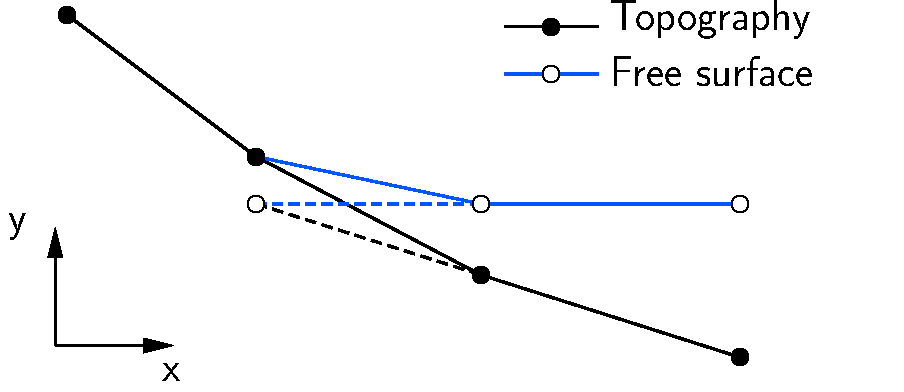
\includegraphics[width=.5\textwidth]{img/fig/partially_dry.pdf}
    \caption{Dry, wet and partially wet elements in the one dimensional case. The dashed line shows the modified topography  and the corresponding free surface.}
    \label{partially_dry}
\end{figure}

\paragraph{Avoiding the singularity of the system matrix}
Since all the elements are included in the computational domain, the last issue to overcome with small water depths is the singularity of the system matrix. The mass balance is satisfied in the dry state, but the momentum equation will become unstable. The easiest (but not more accurate) way to develop a stable scheme is to add a diagonal of non zero terms to the momentum equation:

\begin{equation}
\mathbf{G} \defeq \mathbf{G} + \alpha\,\text{diag}(1, 1, 0)
\end{equation}

The selection of the areas where there is a dry domain is controlled with a wet fraction function. The expression (\ref{h_inv_kurganov}) allows us to define a wet fraction as
\begin{equation}
\eta = hh^{-1}_k
\end{equation}
and
\begin{equation}
\alpha = k(1-\eta)
\end{equation}
In our numerical experiments we have chosen $k=10^3$.



\section{Examples} \label{sec:examples}

This formulation has been implemented in KratosMultiphysics \cite{dadvand2010, dadvand2013}, an open source framework of numerical methods written in C++. Even thought Kratos implements triangles and quadrilaterals with several orders of interpolation \cite{kratos2020}, we have restricted ourselves to linear triangles in order to test the possibilities of the stabilization method. Each example is oriented to test a single aspect of the procedure explained in this research.



\subsection{Wave in a channel with a backward step}

The aim of the first example is to show that the Galerkin formulation applied to the shallow water equations is unstable and how the present stabilization method can overcome this issue and a calibration of the stabilization parameter is performed.
We study the propagation of a wave in a channel with a backward step. The wave is reflected at the end and faces the step in the opposite direction. 

\begin{figure}
    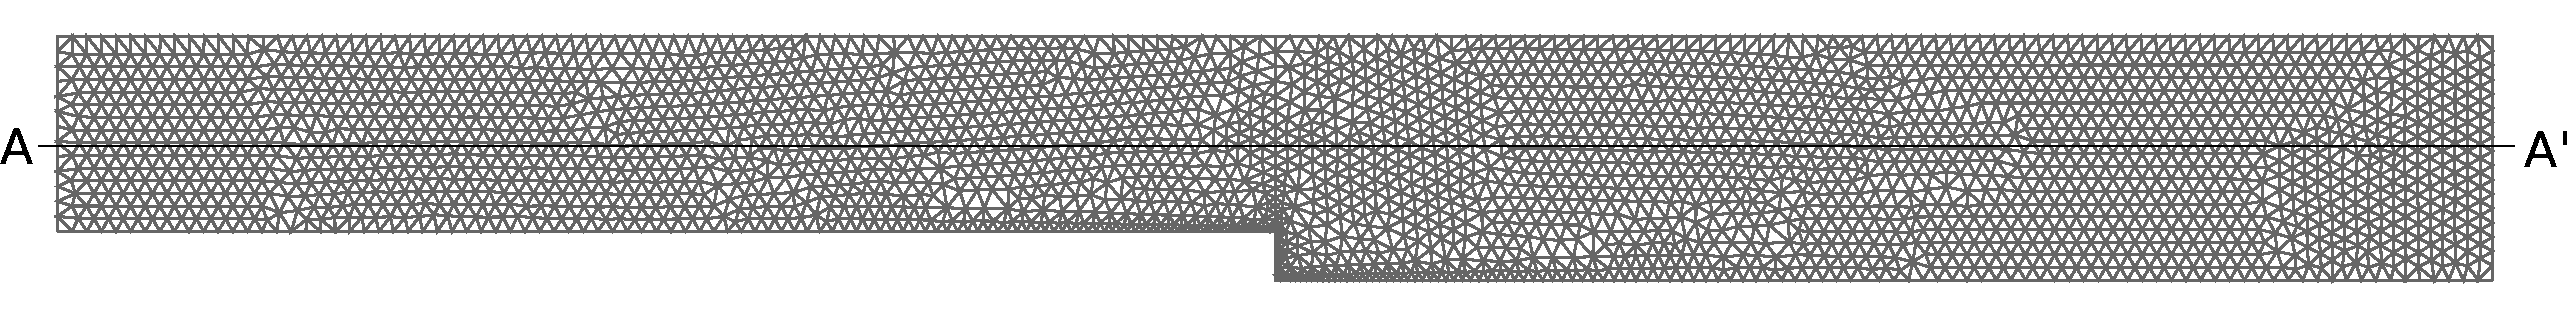
\includegraphics[width=\textwidth]{img/step/mesh.pdf}
    \caption{Definition of the domain and mesh used in the simulation. The average element size is $0.06m$, near the obstacle there is a mesh refinement to $0.02m$. There are $3.125$ nodes and $5.826$ elements.}
    \label{step_mesh}
\end{figure}


\begin{figure}[h]
\begin{subfigure}{\textwidth}
    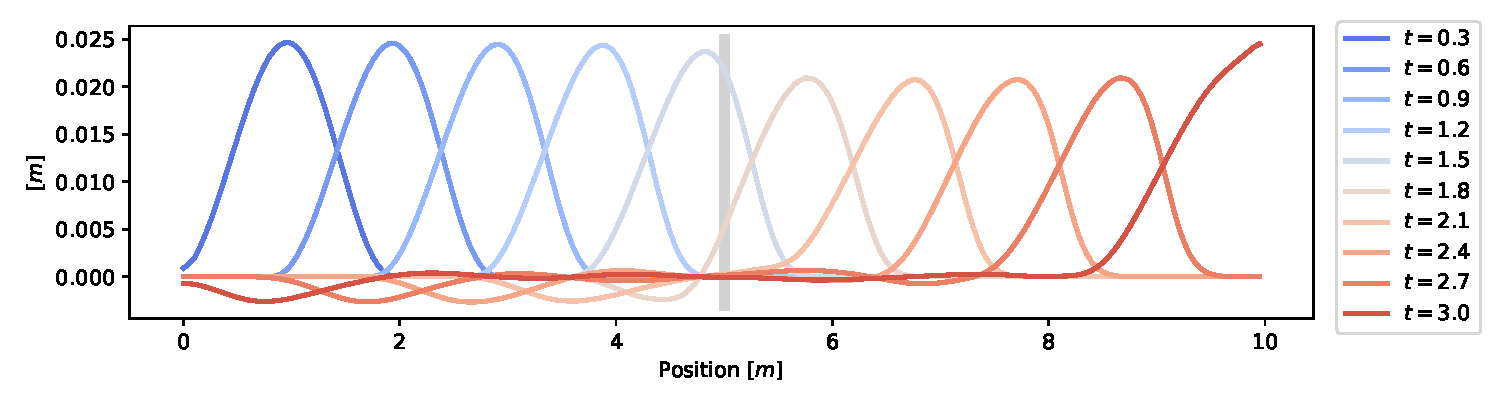
\includegraphics[width=\textwidth]{img/step/free_surface_1.pdf}
\end{subfigure}
\begin{subfigure}{\textwidth}
    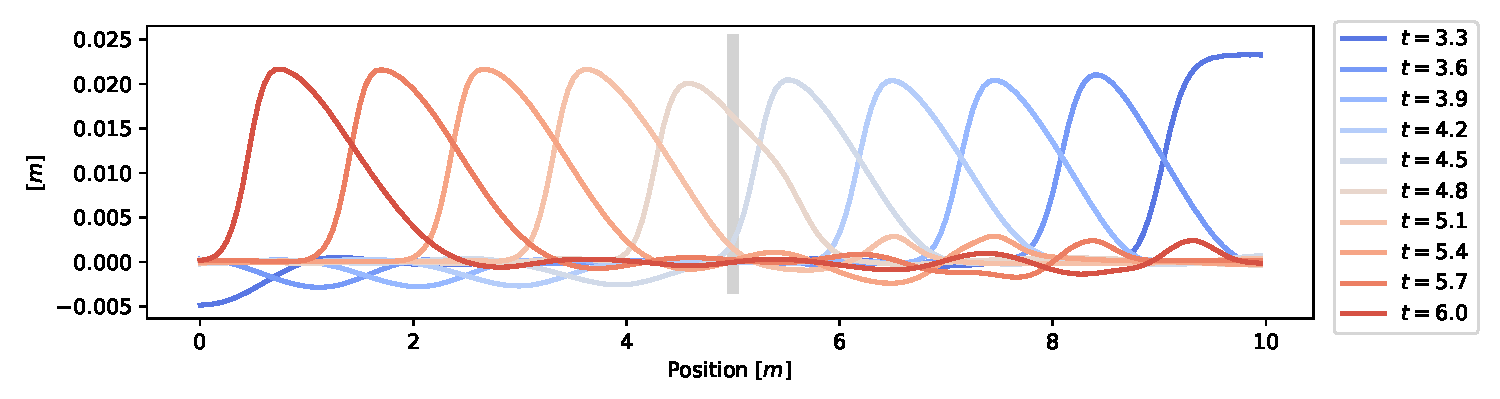
\includegraphics[width=\textwidth]{img/step/free_surface_2.pdf}
\end{subfigure}
\caption{Timestamps of the free surface along the cut AA' from the figure(\ref{step_mesh}). Above the wave is propagating from left to right at times from $0$ to $3s$. The results in the figure below represent the propagation of the reflected wave from right to left at times from $3$ to $6s$.}
\label{waves_propagation}
\end{figure}


\begin{figure}[h]
\begin{subfigure}{.05\textwidth}
    \caption{}
\end{subfigure}
\begin{minipage}[c]{.94\textwidth}
    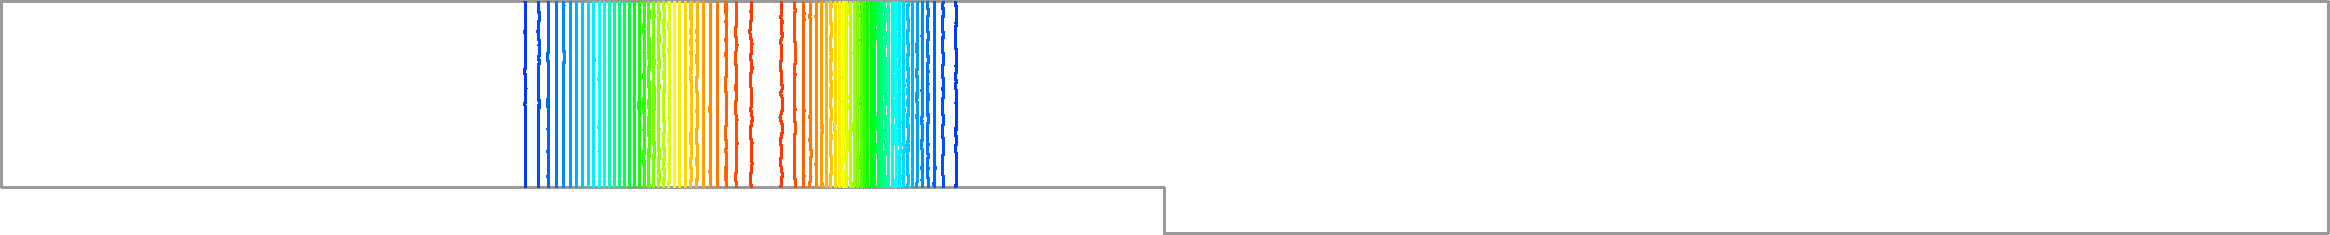
\includegraphics[width=\textwidth]{img/step/stab_0.001_time_1.pdf}        
\end{minipage}
\par\medskip
\begin{subfigure}{.05\textwidth}
    \caption{}
\end{subfigure}
\begin{minipage}[c]{.94\textwidth}
    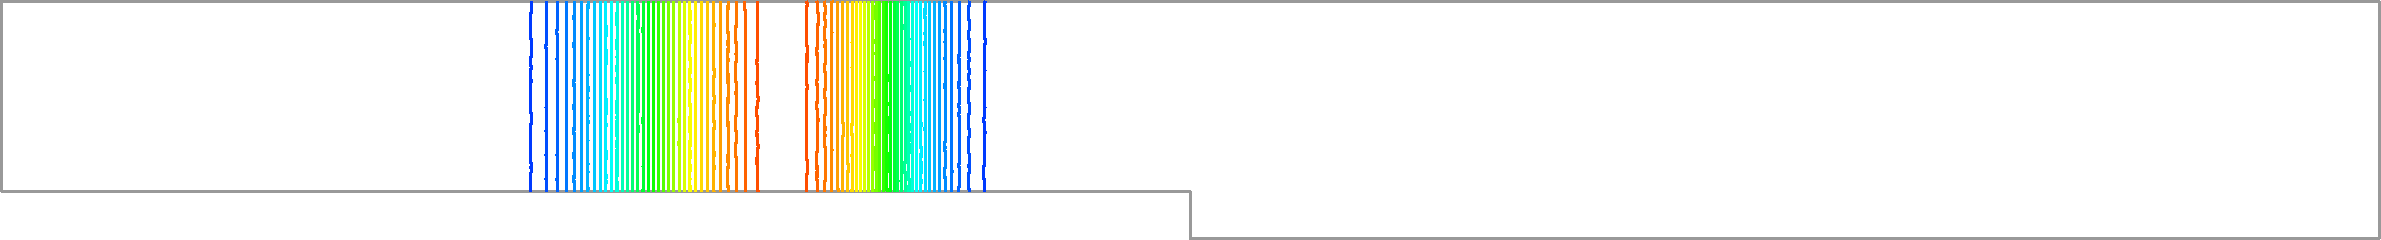
\includegraphics[width=\textwidth]{img/step/stab_0.01_time_1.pdf}        
\end{minipage}
\par\medskip
\begin{subfigure}{.05\textwidth}
    \caption{}
\end{subfigure}
\begin{minipage}[c]{.94\textwidth}
    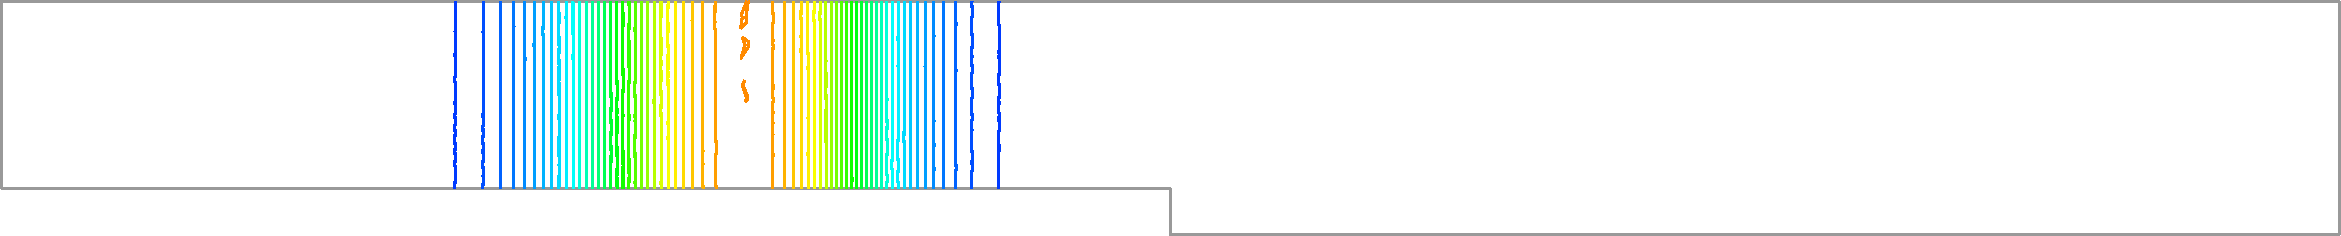
\includegraphics[width=\textwidth]{img/step/stab_0.1_time_1.pdf}        
\end{minipage}
\caption{Contour plots of the free surface elevation at time $t=1s$ for different stabilization factors. The upper figure with $\tau=0.001$ gives an oscillating solution, the middle figure shows a stabilized solution with $\tau=0.01$ and the lower figure shows an over diffusive result with $\tau=0.1$.}
\label{stab_parameters_time1}
\end{figure}

\begin{figure}[h]
    \begin{subfigure}{.05\textwidth}
        \caption{}
    \end{subfigure}
    \begin{minipage}[c]{.94\textwidth}
        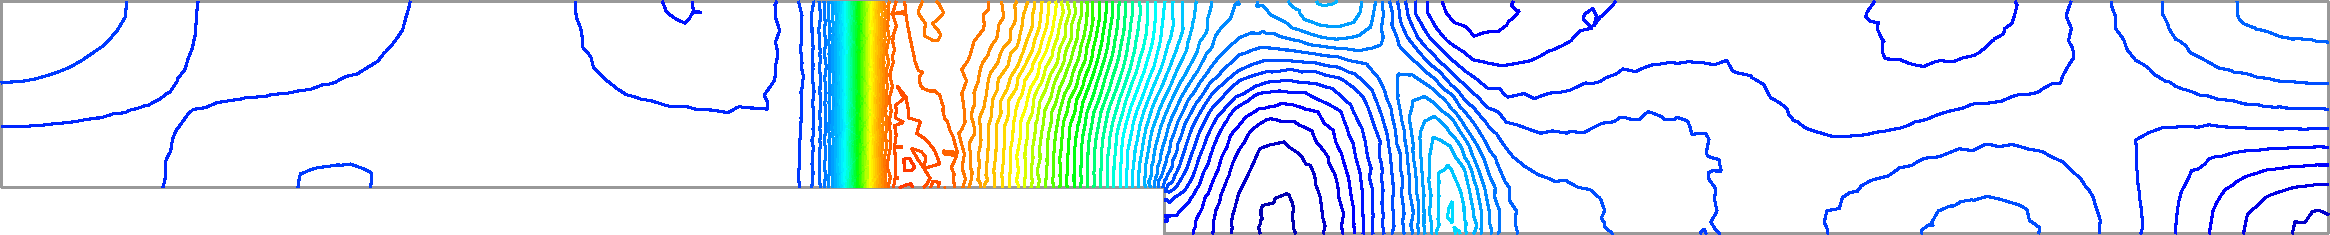
\includegraphics[width=\textwidth]{img/step/stab_0.001_time_5.pdf}        
    \end{minipage}
    \par\medskip
    \begin{subfigure}{.05\textwidth}
        \caption{}
    \end{subfigure}
    \begin{minipage}[c]{.94\textwidth}
        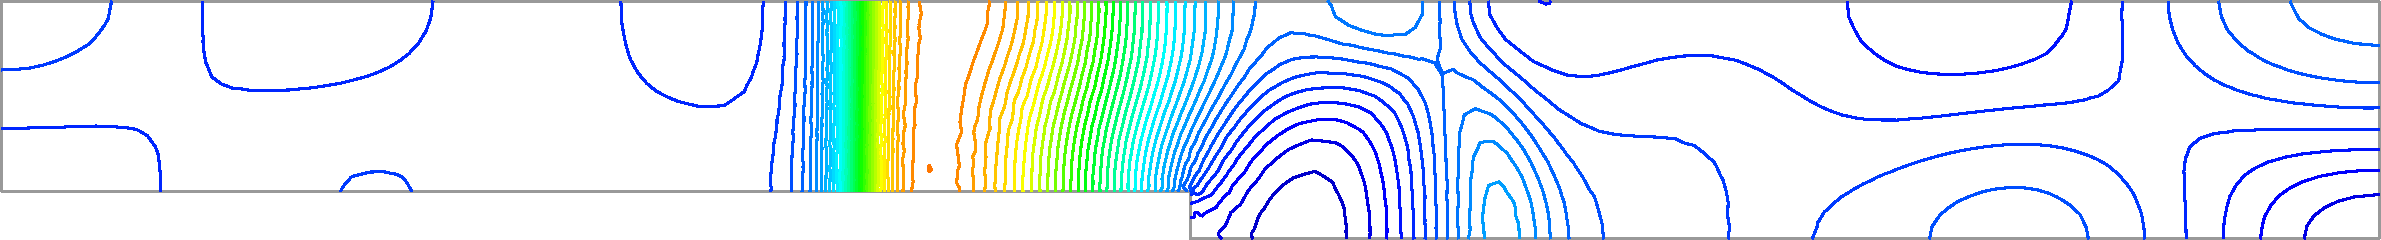
\includegraphics[width=\textwidth]{img/step/stab_0.01_time_5.pdf}        
    \end{minipage}
    \par\medskip
    \begin{subfigure}{.05\textwidth}
        \caption{}
    \end{subfigure}
    \begin{minipage}[c]{.94\textwidth}
        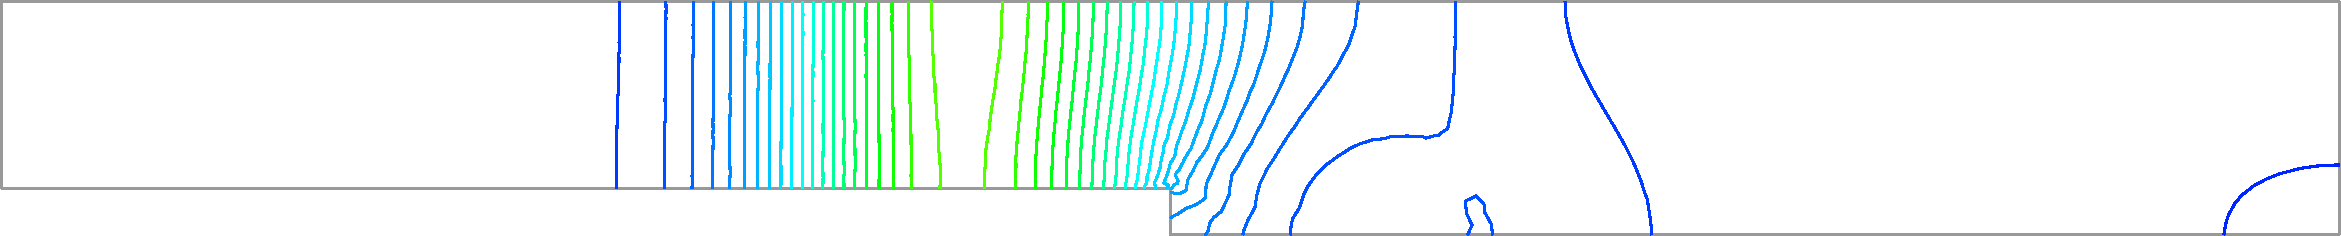
\includegraphics[width=\textwidth]{img/step/stab_0.1_time_5.pdf}        
    \end{minipage}
\caption{Contour plots of the free surface elevation at time $t=5s$ for different stabilization factors. The upper figure with $\tau=0.001$ gives an oscillating solution, the middle figure shows a stabilized solution with $\tau=0.01$ and the lower figure shows an over diffusive result with $\tau=0.1$.}
\label{stab_parameters_time2}
\end{figure}



\subsection{Oscillation in a parabolic basin}

The second example is a classical benchmark oriented to test the accuracy of the location of the moving boundary. The topography follows a parabolic profile while the initial free surface elevation is planar and intersects the topography. The initial configuration corresponds to water at rest but the free surface is in a non horizontal plane. The solution of that problem is an oscillation where the free surface elevation remains planar. An analytical solution can be found in the compilation made by Delestre et al. \cite{delestre2013}.

The domain $\Omega$ is defined in the interval $[0,L]\times[0,1]m$ where $L=10$ and all the boundaries are reflective ($\mathbf{u}\cdot\mathbf{n} = 0$). The topography is given by the following expression
\begin{equation}
z(x,y) = h_0 \left(\frac{1}{a^2}\left(x - \frac{L}{2}\right)^2 - 1\right)
\end{equation}
and the primitive variables are defined by
\begin{subequations}
\begin{align}
h(x,y) &=
\begin{cases}
-h_0\left(\left(\frac{1}{a}\left(x - \frac{L}{2}\right) + \frac{1}{2a}\cos(2Bt)\right)^2 - 1\right)
\quad &\text{if} \ x_1(t) < x < x_2(t) \\
0 \quad &\text{otherwise}
\end{cases} \\
\mathbf{u}(x,y) &=
\begin{cases}
(B,0)\sin(2Bt) \quad &\text{if} \ x_1(t) < x < x_2(t) \\
(0,0) \quad &\text{otherwise}
\end{cases}
\end{align}
\end{subequations}
where $B=\sqrt{2gh_0}/2a$, and $x_1$, $x_2$ are time dependent functions which define the location of the dry-wet interface:
\begin{equation}
\begin{split}
x_1(t) = -\frac{1}{2}\cos(2Bt) - a + \frac{L}{2} \\
x_2(t) = -\frac{1}{2}\cos(2Bt) + a + \frac{L}{2}
\end{split}
\end{equation}


\begin{figure}[H]
\begin{subfigure}{\textwidth}
    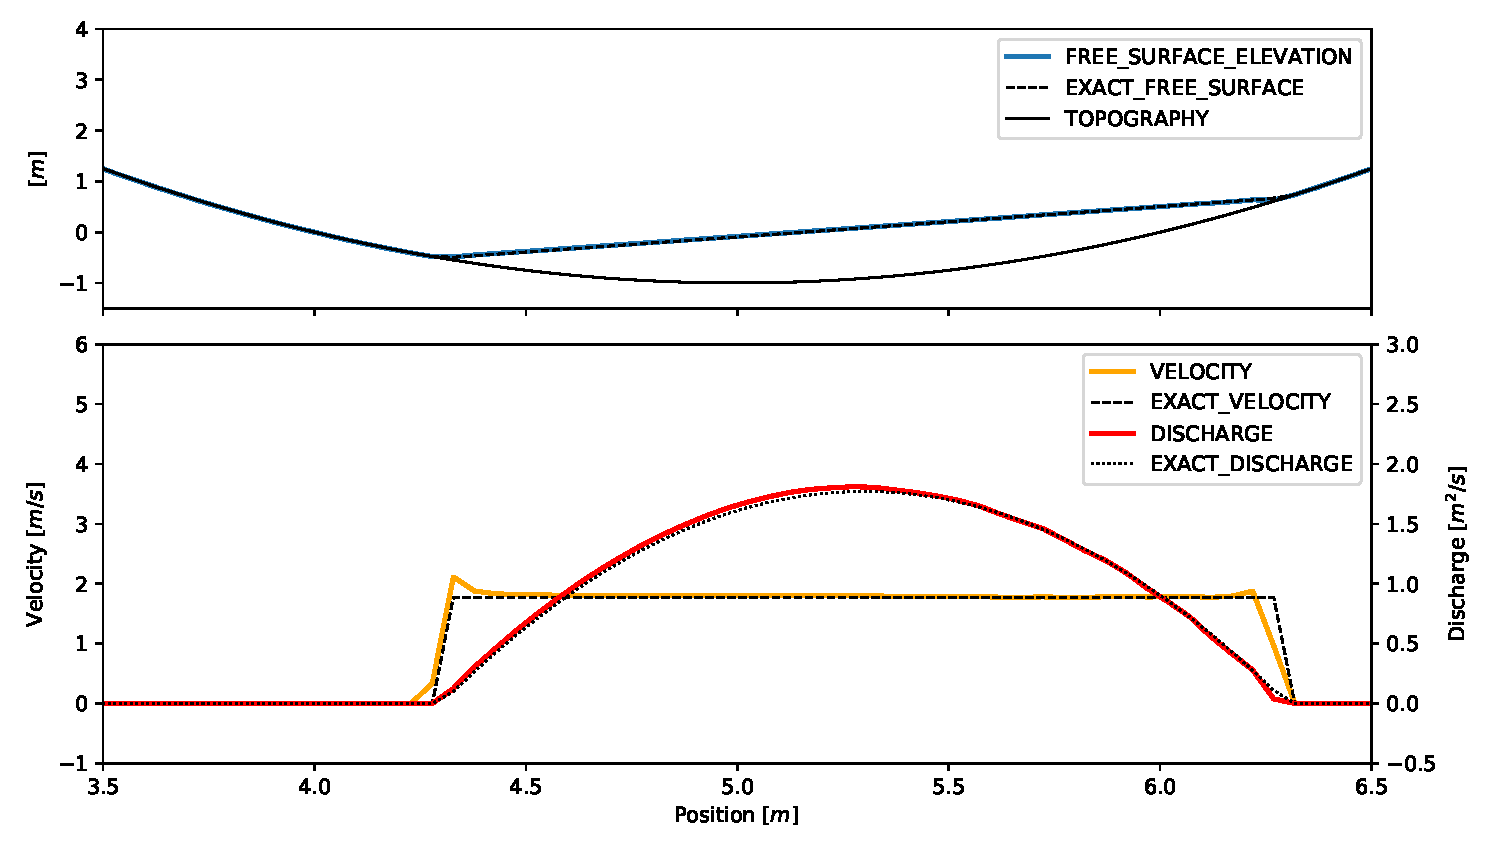
\includegraphics[width=\textwidth]{img/par/parabola_t0.5.pdf}
\end{subfigure}
\par\medskip
\begin{subfigure}{\textwidth}
    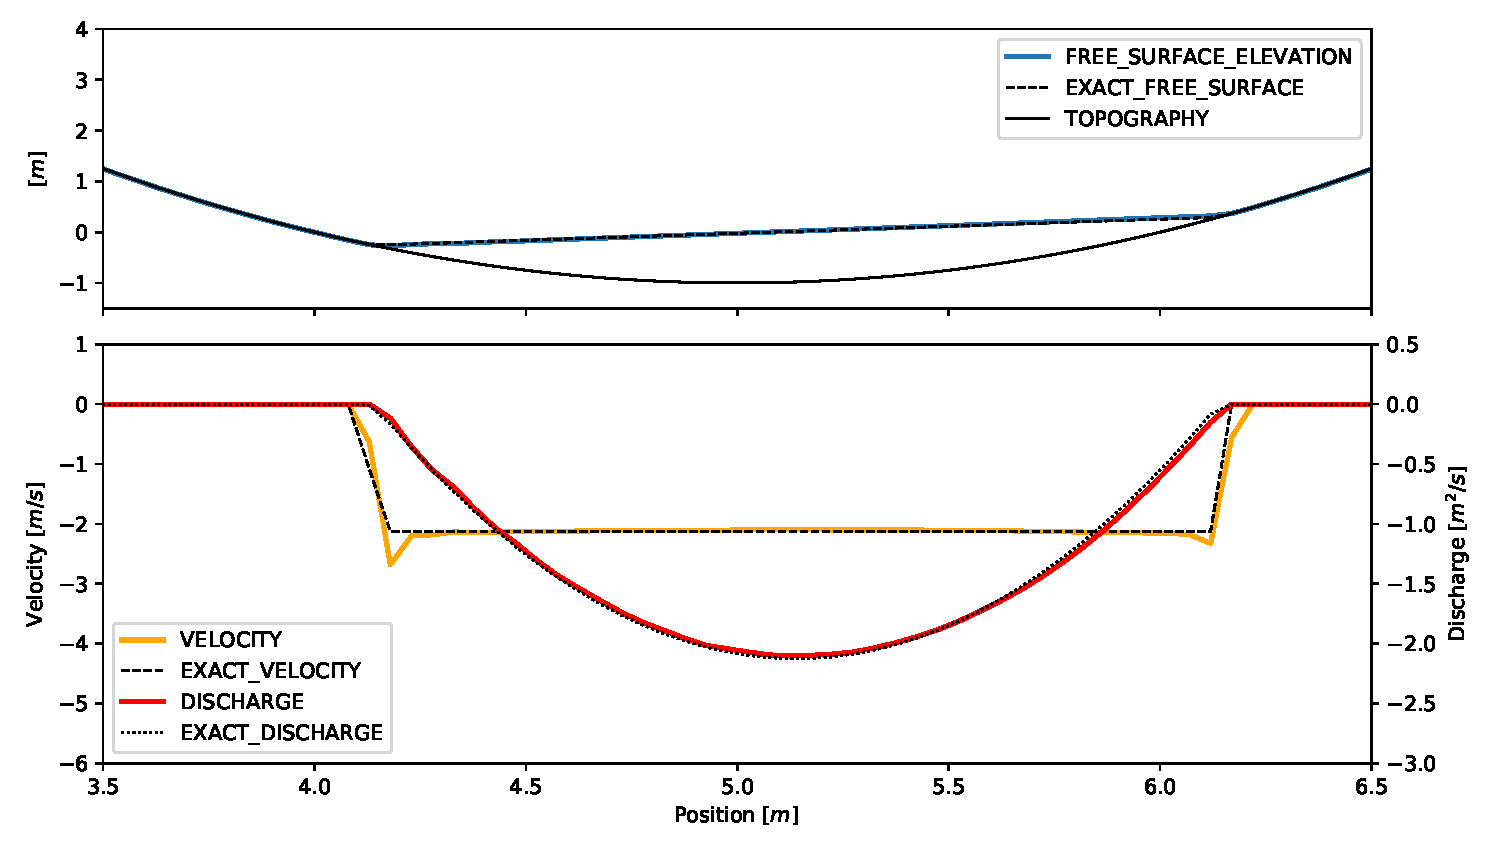
\includegraphics[width=\textwidth]{img/par/parabola_t1.0.pdf}
\end{subfigure}
\caption{Cuts along the mesh of size $0.03m$ at times $=0.5s$ (above) and $t=1s$ (below). There are 333 nodes along the cut.}
\label{parabola_graphic}
\end{figure}

\begin{figure}[H]
\begin{subfigure}{\textwidth}
    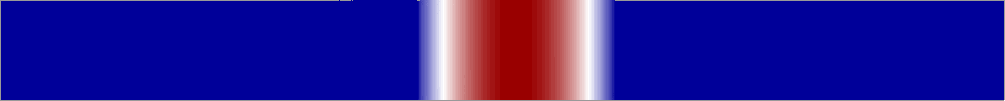
\includegraphics[width=\textwidth]{img/par/height_1.0.png}
\end{subfigure}
\par\medskip
\begin{subfigure}{\textwidth}
    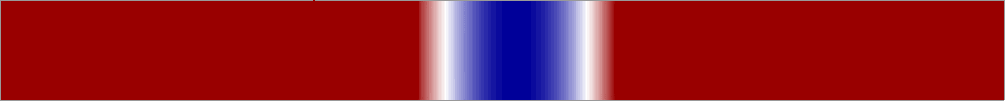
\includegraphics[width=\textwidth]{img/par/momentum_1.0.png}
\end{subfigure}
\par\medskip
\begin{subfigure}{\textwidth}
    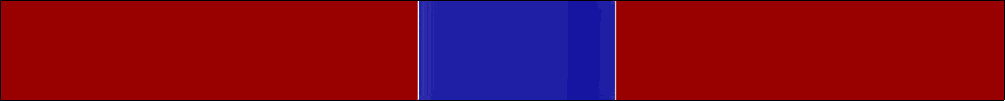
\includegraphics[width=\textwidth]{img/par/velocity_1.0.png}
\end{subfigure}
\caption{Results with the fie mesh of size $0.01m$ at time $t=1s$. The images display the water height at the top, the x-discharge at the middle and the x-velocity below. There is not legend for simplicity, the red colour is positive and blue means a null or negative magnitude.}
\label{parabola_results}
\end{figure}

\begin{figure}[H]
\begin{subfigure}{0.4\textwidth}
    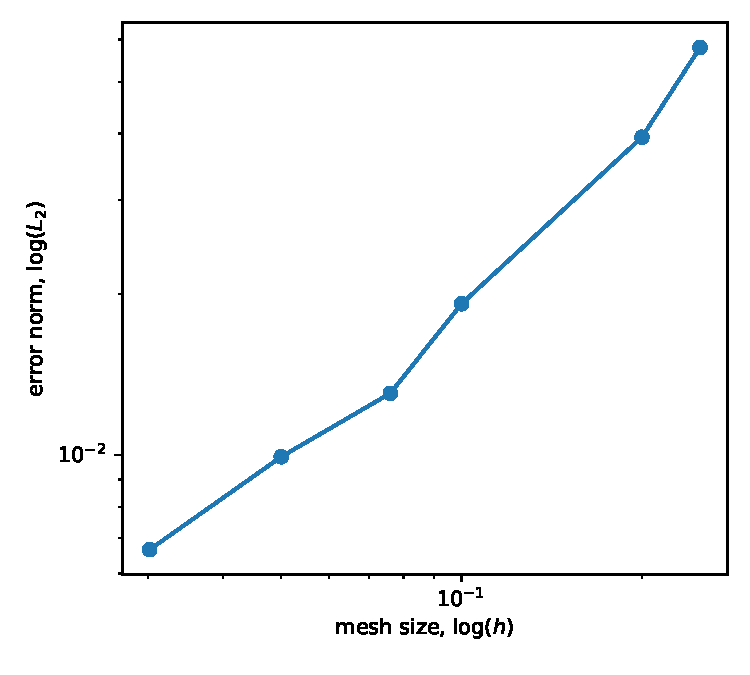
\includegraphics[width=\textwidth]{img/par/conv_1.pdf}    
\end{subfigure}
\hfill
\begin{subfigure}{0.58\textwidth}
    \begin{tabular}{+>{\small}r^c^c^c^c} \hline
    $n_{nodes}$ & $\Delta x$ & $\Delta t$ & CFL & $L_2(e_{rel})$ \\ \hline
    205     & 0.25  &  0.002 & 0.041 & 0.211 \\ %0.0760 \\
%    306     & 0.2   &  0.002 & 0.051 & 0.138 \\ %0.0496 \\
    1,111   & 0.1   &  0.002 &  0.10 & 0.106 \\ %0.0382 \\
%    1,876   & 0.075 &  0.002 &  0.14 & 0.0619 \\ %0.0223 \\
    4,221   & 0.05  &  0.002 &  0.21 & 0.0336 \\ %0.0121 \\
\rowstyle{\bfseries}
    4,221   & 0.05  &  0.004 &  0.42 & 0.0347 \\ %0.0113 \\
    11,356  & 0.03  &  0.002 &  0.34 & inf \\
    101,101 & 0.01  &  0.0005 &  0.26 & inf \\ \hline
    \end{tabular}
\end{subfigure}
\caption{Convergence analysis for the parabolic basin benchmark}
\label{parabola_convergence}
\end{figure}



\subsection{Short channel with smooth transition and shock}

The third example in a benchmark based on the Mac Donald's type solutions \cite{macdonald1997}. The analytical solution also can be found in the same compilation than the previous example \cite{delestre2013}. This test presents channel with a steady state solution. There is a subcritical inlet in a region where a transcritical flow is produced. The outlet is also subcritical and a shock is generated at $\sfrac{2}{3}$ of the channel. The aim of this example is to evaluate the presented shock capturing technique and the correct location of the hydraulic jump.

Here we will consider the one-dimensional shallow water equations without diffusion and only with Manning bottom friction as source term. A steady state solution satisfies $\pder{q}{x}=0$ and the equation (\ref{general_sw}) reduces to
\begin{equation} \label{steady_state}
\pder{z}{x} = \left(\frac{v^2}{gh}-1\right) \pder{h}{x} - n^2\frac{\abs{v}v}{h^{\sfrac{4}{3}}}
\end{equation}
This relation allows to integrate the topography given an analytical expression for the water height. Another approach in hydraulics is to consider a given discharge and topography and integrate the water height using the relation (\ref{steady_state}). In both approaches exact solutions can be obtained. Since this expression involves the bottom friction, we can prove if the friction term is coded in order to satisfy the steady state.

For this benchmark we have considered the domain defined by the interval $[0,100]\times[0,5]$ which is a channel of $100m$ length and $5m$ width, and the following boundary conditions:
\begin{equation}
\begin{split}
    q_x = 2\ \text{m/s} \qquad &\text{in} \ \Gamma_{upstream} \\
    h = h_{ex}(100) \qquad &\text{in} \ \Gamma_{downstream} \\
    q_y = 0 \qquad &\text{in} \ \Gamma_{walls}
\end{split}
\end{equation}
The Manning coefficient is $0.0328\ \text{m}^{-1/3}\text{s}$ and the water height $h_{ex}(x)$ is a piecewise function defined in \cite{delestre2013}. The discontinuity of the water height function is located at $x=200/3\ m$ and defines the hydraulic jump.

\begin{figure}
    
\includegraphics[width=\textwidth]{img/jump/sketch/sketch.pdf}
    \caption{Geometry of the channel, the vertical line shows the position of the hydraulic jump, the shadowed area correspond to the location where the $L_2$ norm of the error is computed.}
\end{figure}


\begin{figure}[H]
\begin{subfigure}{0.4\textwidth}
    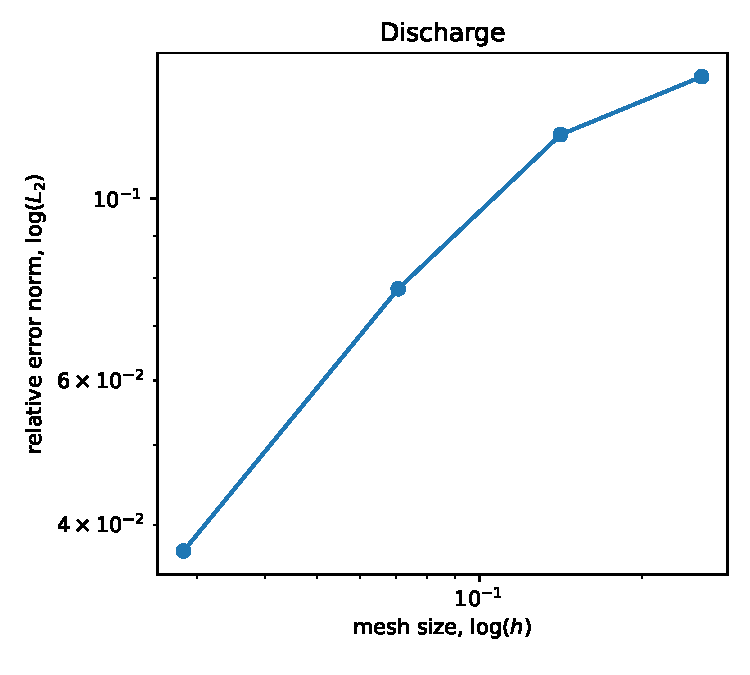
\includegraphics[width=\textwidth]{img/jump/momentum_convergence.pdf}    
\end{subfigure}
\hfill
\begin{subfigure}{0.58\textwidth}
    \begin{tabular}{+>{\small}r^c^c^c^c} \hline
    $n_{nodes}$ & $\Delta x$ & $\Delta t$ & CFL   & $L_2(e_{rel})$ \\ \hline
    204         &        2.0 &      0.005 & 0.016 & 0.177 \\
    606         &        1.0 &      0.005 & 0.031 & 0.138 \\
    2211        &        0.5 &      0.005 & 0.062 & 0.088 \\
    13026       &        0.2 &      0.005 & 0.15  & 0.041 \\ \hline
    \end{tabular}
\end{subfigure}
\caption{Convergence analysis for the short channel with smooth transition and shock.}
\label{hydraulic_jump_convergence}
\end{figure}

% \begin{figure}[H]
%     \begin{subfigure}{.49\textwidth}
%         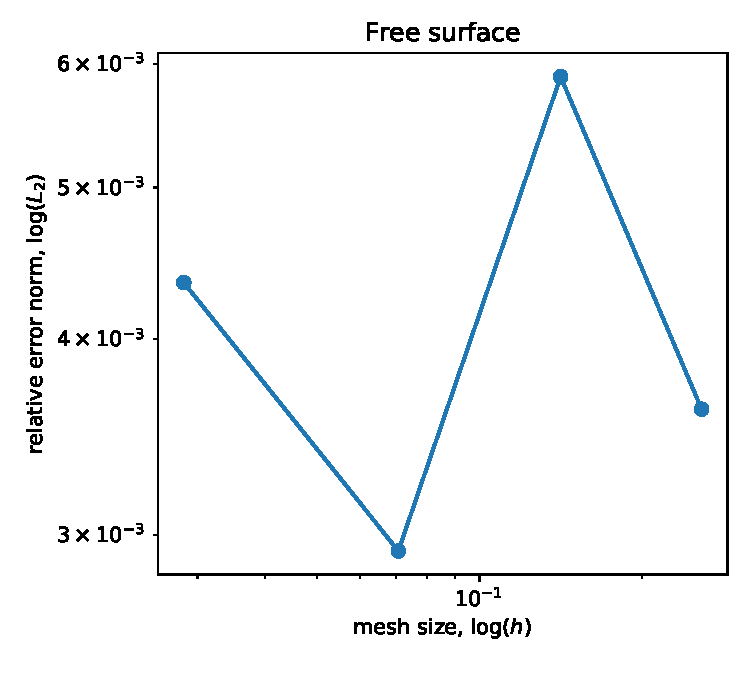
\includegraphics[width=\textwidth]{img/jump/height_convergence.pdf}
%     \end{subfigure}
%     \hfill
%     \begin{subfigure}{.49\textwidth}
%         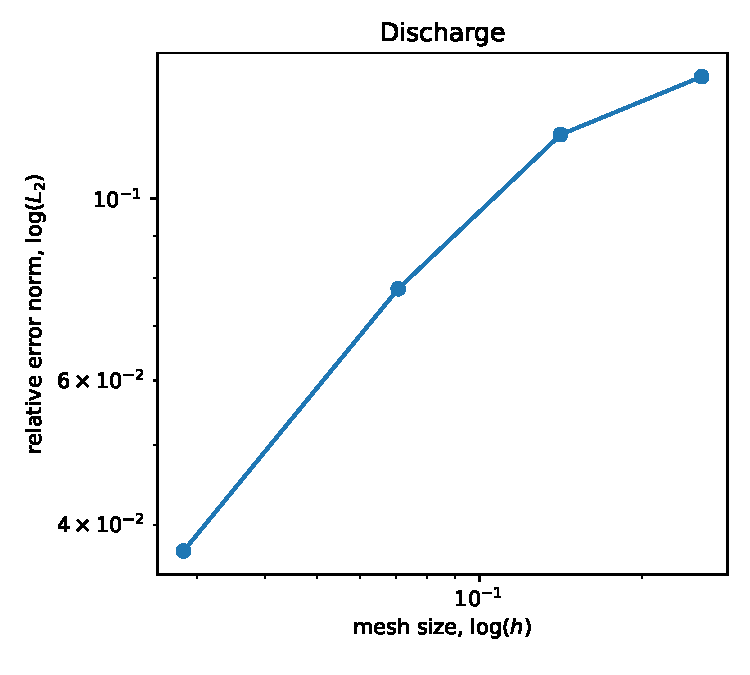
\includegraphics[width=\textwidth]{img/jump/momentum_convergence.pdf}
%     \end{subfigure}
%     \caption{Convergence graphics for the water height (left) and discharge (right) for the short channel with smooth transition and shock.}
%     \label{mac_donald_shock_convergence}
% \end{figure}

\begin{figure}
    \centering
    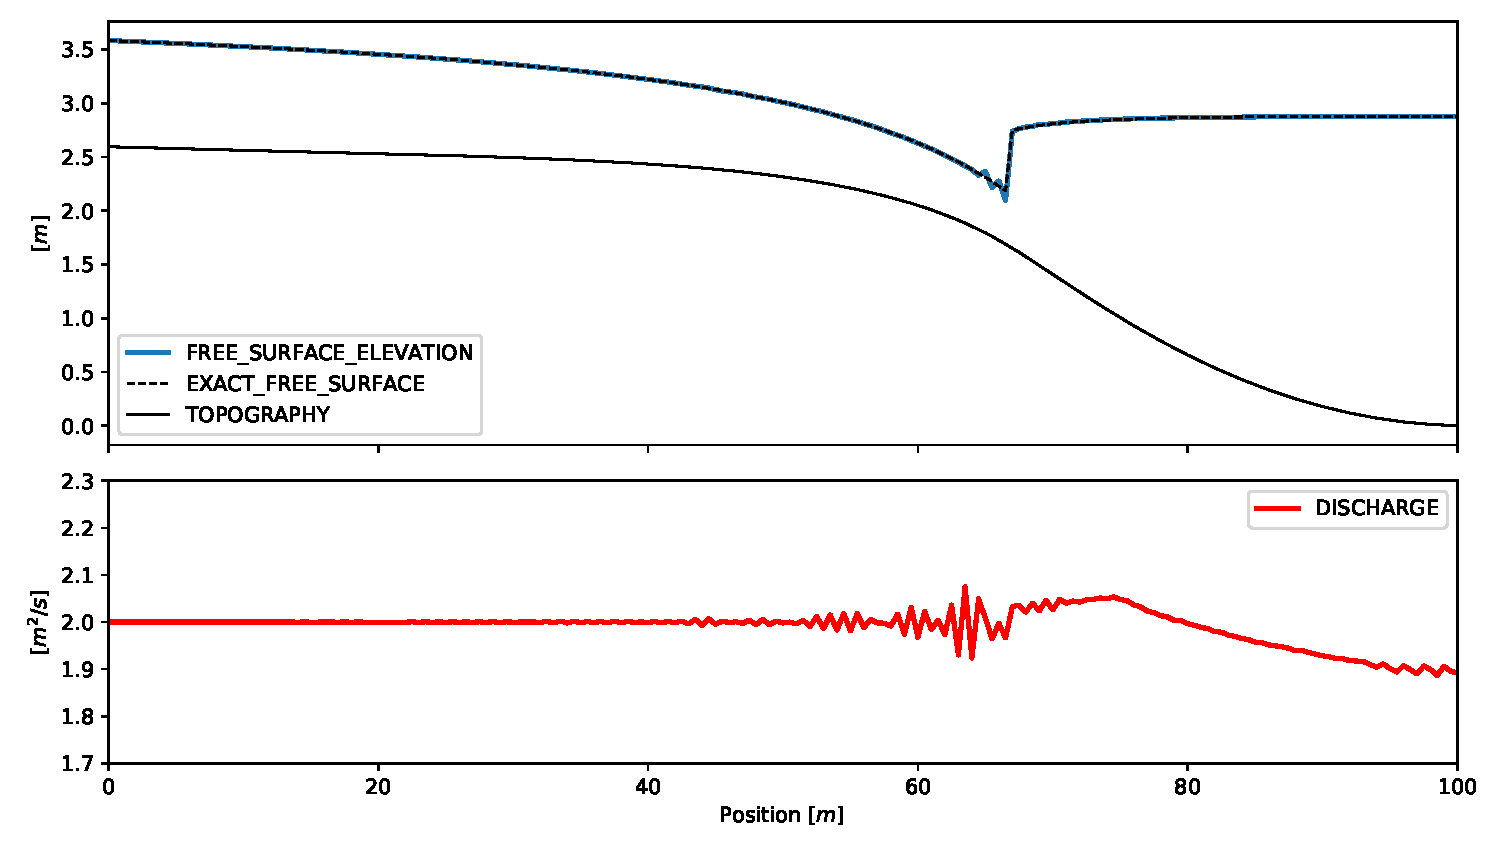
\includegraphics[width=\textwidth]{img/jump/mesh_0.5.pdf}
    \caption{Graph along the cut defined by the center of the channel. The mesh size is $0.5m$}
    \label{mac_donald_shock_graph_5}
\end{figure}

\begin{figure}
    \centering
    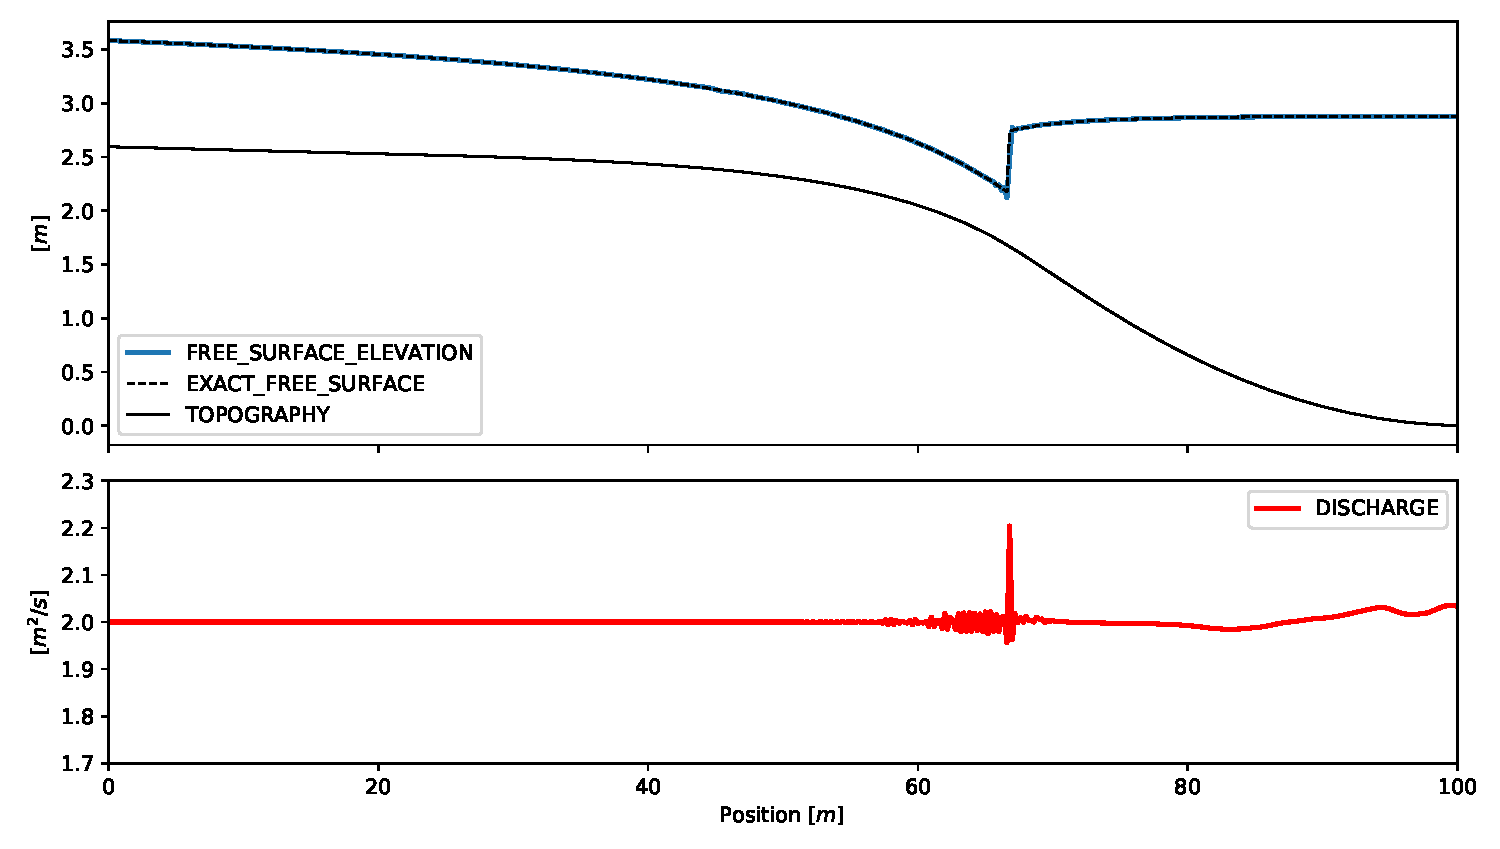
\includegraphics[width=\textwidth]{img/jump/mesh_0.2.pdf}
    \caption{Graph along the cut defined by the center of the channel. The mesh sie is $0.2m$}
    \label{mac_donald_shock_graph_2}
\end{figure}


\subsection{Experiment}

The last example consist on the reproduction of the experiment carried out by Soares \cite{soares2007}. A dam break flow with a building downstream is simulated and the problem definition is depicted in figure \ref{experiment_sketch}. The channel is $3.4m$ width and the end of the dam is located at $x=0$. As initial conditions, the water depth is set to $0.4m$ in the reservoir and the channel is dry. The manning coefficient is $0.01ms^{-1}$ over all the domain. At the beginning of the simulation, the gate of the dam is removed and the water is allowed to flow around the building.

Figure \ref{experiment_plots} shows several results of the water depth after the gate release and figure \ref{experiment_gauges} shows the evolution of the water depth at the gauges.
Regarding the performance of that formulation, it captures the main aspects of the flow, but not the details, since there are some regions on that experiment which violate the shallow water approximations.

\begin{figure}[H]
\centering
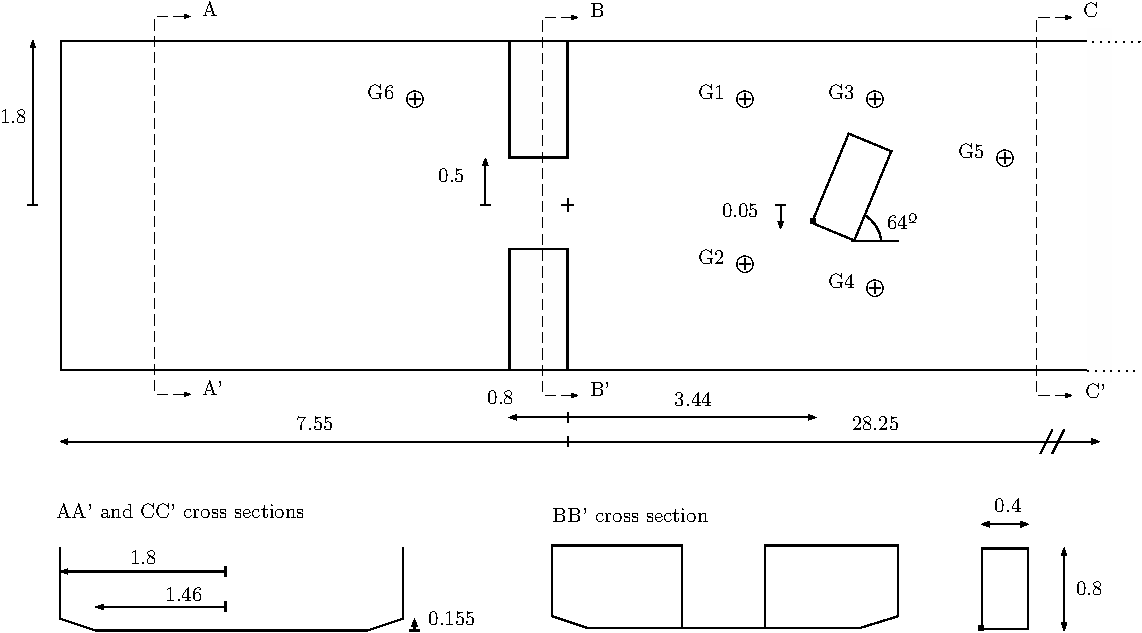
\includegraphics[width=\textwidth]{img/exp/sketch.pdf}
\caption{Definition of the isolated building benchmark. The dimensions are in $m$.}
\label{experiment_sketch}
\end{figure}


\begin{figure}[H]
\centering
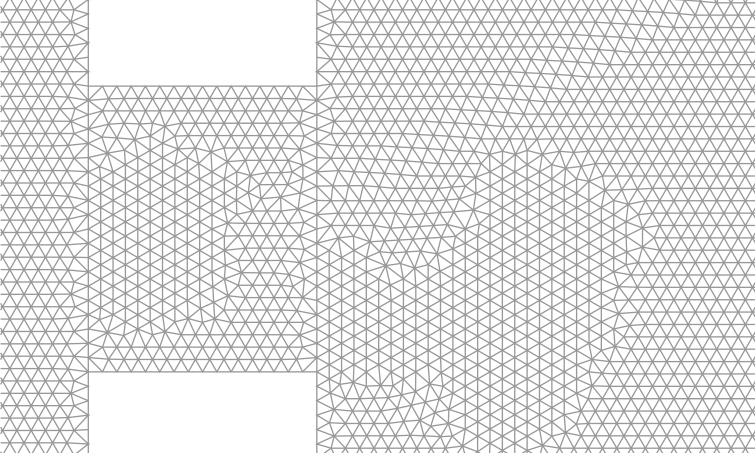
\includegraphics[width=.49\textwidth]{img/exp/mesh_dam.png}
\hfill
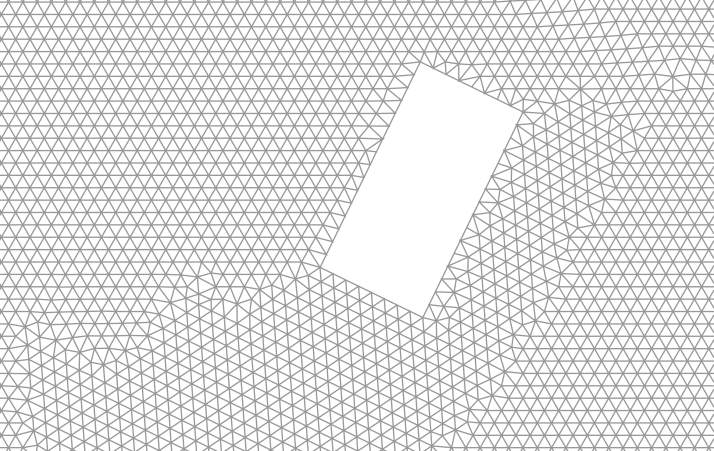
\includegraphics[width=.47\textwidth]{img/exp/mesh_building.png}
\caption{Details of the mesh around the dam and around the building. The average mesh size is $0.05m$ and there are 115.000 elements.}
\label{experiment_mesh}
\end{figure}


\begin{table}
\centering
\begin{tabular}{ccc}
\hline
Gauge number & X & Y \\ \hline
1 &  2.65 &  1.15 \\
2 &  2.65 & -0.60 \\
3 &  4.00 &  1.15 \\
4 &  4.00 & -0.80 \\
5 &  5.20 &  0.30 \\
6 & -1.87 &  1.10 \\ \hline
\end{tabular}
\caption{Positions of the gauges, units in $m$.}
\label{gauges_positions}
\end{table}


\begin{figure}
\centering
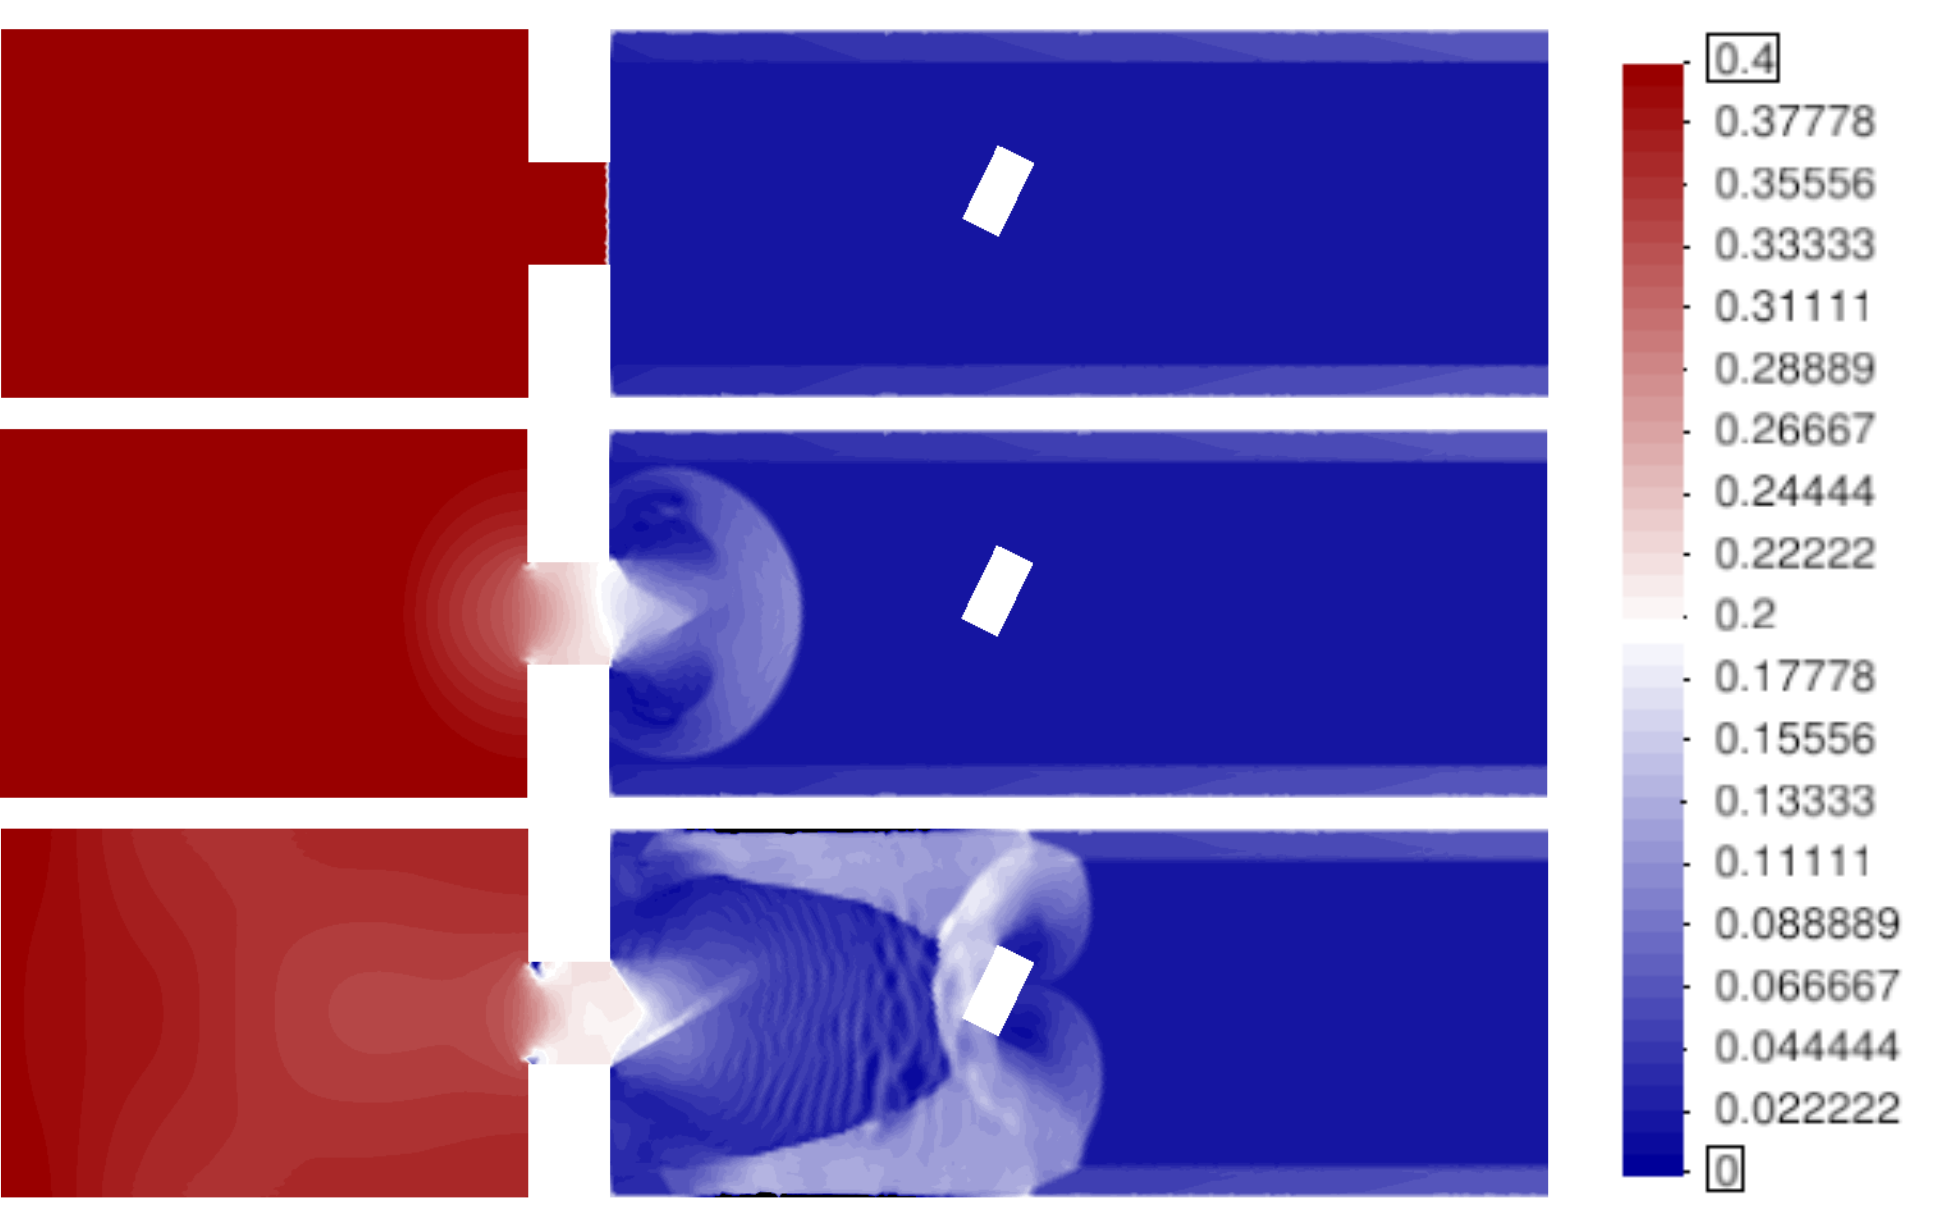
\includegraphics[width=\textwidth]{img/exp/results.png}
\caption{Results of the benchmark at times $0$, $1$ and $3$ seconds}
\label{experiment_plots}
\end{figure}


\begin{figure}
\centering
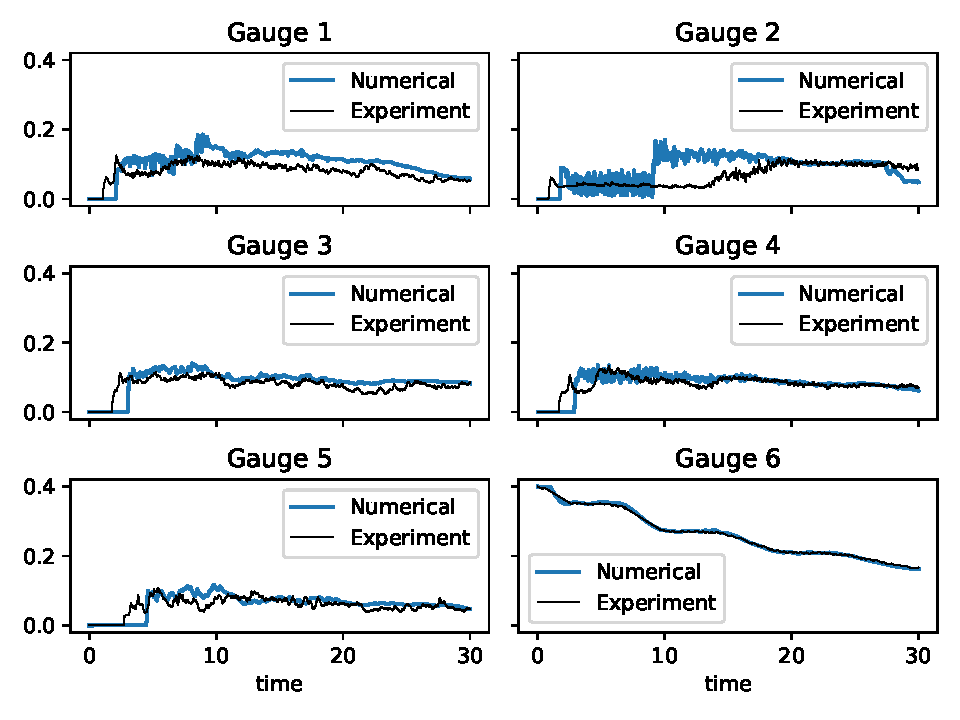
\includegraphics[width=\textwidth]{img/exp/gauges.pdf}
\caption{Comparison between the obtained water depth with the reference data.}
\label{experiment_gauges}
\end{figure}

\section{Concluding remarks} \label{sec:conclusions}


\section*{Appendix A}
\addcontentsline{toc}{section}{Appendix A}

The stabilization matrices ere the result of multiplying $\mathbf{A}$ tensor by itself:

\begin{subequations}
\begin{equation}
\mathbf{A}_1\mathbf{A}_1 =
\begin{pmatrix}
3u_1^2 + c^2 & 0  & -2u_1^3 + 2u_1c^2 \\
2u_1u_2  & u_1^2  & -2u_1^2u_2 + u_2c^2 \\
2u_1  & 0   & -u_1^2 + c^2
\end{pmatrix}
\end{equation}
\begin{equation}
    \mathbf{A}_2\mathbf{A}_2 =
\begin{pmatrix}
u_2^2  & 2u_1u_2  & -2u_1u_2^2 + u_1c^2 \\
0    & 3u_2^2 + c^2 & -2u_2^3 + 2u_2c^2 \\
0  & 2u_2  & -u_2^2 + c^2
\end{pmatrix}
\end{equation}
\begin{equation}
\mathbf{A}_1\mathbf{A}_2 =
\begin{pmatrix}
2u_1u_2  & u_1^2 + c^2  & -2u_1^2u_2 \\
u_2^2  & 2u_1u_2  & -2u_1u_2^2 + u_1c^2 \\
u_2  & u_1  & -u_1u_2
\end{pmatrix}
\end{equation}
\begin{equation}
\mathbf{A}_2\mathbf{A}_1 =
\begin{pmatrix}
2u_1u_2  & u_1^2  & -2u_1^2u_2 + u_2c^2 \\
u_2^2 + c^2  & 2u_1u_2  & -2u_1u_2^2 \\
u_2  & u_1  & -u_1u_2
\end{pmatrix}
\end{equation}
\end{subequations}


\bibliography{../bibliography/sw}
\bibliographystyle{ieeetr}

\end{document}
